\documentclass{article}
%\usepackage[english]{babel}%
\usepackage{graphicx}
\usepackage{tabulary}
\usepackage{tabularx}
\usepackage[table,xcdraw]{xcolor}
\usepackage{pdflscape}
%\usepackage{gensymb}
\usepackage{lastpage}
\usepackage{multirow}
\usepackage{xcolor}
\usepackage{cancel}
\usepackage{amsmath}
\usepackage[table]{xcolor}
\usepackage{fixltx2e}
\usepackage[T1]{fontenc}
\usepackage[utf8]{inputenc}
\usepackage{ifthen}
\usepackage{fancyhdr}
\usepackage[utf8]{inputenc}
\usepackage{tikz}
\usepackage[document]{ragged2e}
\usepackage[margin=1in,top=1.2in,headheight=57pt,headsep=0.1in]
{geometry}
\usepackage{ifthen}
\usepackage{fancyhdr}
\everymath{\displaystyle}
\usepackage[document]{ragged2e}
\usepackage{fancyhdr}
\usepackage{mathabx}
\usepackage{textcomp,mathcomp}
\usepackage[shortlabels]{enumitem}
\everymath{\displaystyle}
\linespread{2}%controls the spacing between lines. Bigger fractions means crowded lines%
\linespread{1.3}%controls the spacing between lines. Bigger fractions means crowded lines%
\pagestyle{fancy}
\setlength{\headheight}{56.2pt}
\usepackage{soul}
\usepackage{siunitx}

%\usepackage{textcomp}
\usetikzlibrary{shapes.multipart, shapes.geometric, arrows}
\usetikzlibrary{calc, decorations.markings}
\usetikzlibrary{arrows.meta}
\usetikzlibrary{shapes,snakes}
\usetikzlibrary{quotes,angles, positioning}
%\chead{\ifthenelse{\value{page}=1}{\includegraphics[scale=0.3]{BassettCTCLogo}}}
%\rhead{\ifthenelse{\value{page}=1}{Final Exam}{}}
%\lhead{\ifthenelse{\value{page}=1}{Water Treatment - Oct-Dec 2022}{\textbf Final Exam}}
%\rfoot{\ifthenelse{\value{page}=1}{}{}}
%
%\cfoot{}
%\lfoot{Page \thepage\ of \pageref{LastPage}}
%\renewcommand{\headrulewidth}{2pt}
%\renewcommand{\footrulewidth}{1pt}
\begin{document}
\section*{Density}\index{Density}
\begin{itemize}
\item Density is defined as the weight of a substance per a unit of its volume. For example, pounds per cubic foot or pounds per gallon.

\item Here are a few key facts about density:
\begin{itemize}

\item Density is measured in units of lb/ft3, lb/gal, or mg/L. Density of water = 62.4 lb/ft3 = 8.34 lb/gal.
\end{itemize}
\end{itemize}

\section*{Specific Gravity}\index{Specific Gravity}
\begin{itemize}
\item Specific gravity is the ratio of the density of a substance (liquid or solid) to the density water.
\item It is the ratio of the weight of the substance of a certain volume to the weight of water of the same volume.

\item Any substance with a density greater than that of water will have a specific gravity greater than 1.0. Any substance with a density less than that of water will have a specific gravity less than 1.0. 

\item Specific gravity examples:
\begin{itemize}

\item Specific gravity of water = 1.0 
\item Specific gravity of concrete = 2.5 (depending on ingredients)
\item Specific gravity of alum (liquid @ 60°F) = 1.33 
\item Specific gravity of hydrogen peroxide (35\%) = 1.132
\end{itemize}

\item Specific gravity is used in two ways:
\begin{enumerate}
\item To calculate the total weight of a \% solution (either as a single gallon or a drum volume).\\
Total Weight = Drum Vol X SG X 8.34
\item To calculate the “active ingredient” weight of a single gallon or a drum.\\

Active Ingredient Weight within Drum = Drum Volume X SG X 8.34 X \% solution as a decimal. (i.e., Total Weight X \% solution as a decimal)\\

NOTE: Both ways start with solving for the total weight (Drum Vol X SG X 8.34). When solving for “active ingredient” weight, you have to then multiply by \% solution as a decimal.

\end{enumerate}
\end{itemize}

\textbf{Example:} What is the weight of 5 gallons of a 40\% ferric chloride solution given its specific gravity of 1.43?
$$(8.34 * 1.43) \enspace lbs/gal*5 \enspace gallons = \boxed{59.6 \enspace lbs}$$

The weight of active ferric chloride in the drum will be 59.6*0.4=23.84 lbs (as ferric chloride is 40\% strength)

% \begin{tcolorbox}[
% colframe=blue!25,
% colback=blue!10,
% coltitle=blue!20!black,  
% title= Practice Problems]
% \begin{enumerate}
% \item What is the specific gravity of a 1 ft$^3$ concrete block which weighs 145 lbs?

% \item What is the specific gravity of a chlorine solution if 1 (one) gallon weighs 10.2lbs?

% \item How much does each gallon of zinc orthophosphate weigh (pounds) if it has a specific gravity of 1.46?

% \item How much does a 55 gallon drum of 25\% caustic soda weigh (pounds) if the specific gravity is 1.28?

% \end{enumerate}

% \end{tcolorbox}


\section*{Concentration}\index{Concentration}
\begin{itemize}
\item Concentration is typically expressed as mg/l which is the weight of the constituent (mg) in 1 liter of water.
\item As 1 liter of water weighs 1 million mg, a concentration of 1 mg/l implies 1 mg of constituent per 1 million mg of water or one part per million (ppm).   \texthl{Thus, mg/l and ppm are synonymous.}
\item Sometimes the constituent concentration is expressed in terms of percentage.\\
\vspace{6pt}
\textbf{Example:} 12.5\% chlorine concentration solution.\\
\vspace{0.2cm}
100\% would mean 1,000,000 mg/l or 1,000,000 ppm\\
\vspace{0.2cm}
$\implies$1\% would be $\dfrac{1,000,000}{100}\textrm{mg/l} = \textrm{10,000 mg/l or 10,000 ppm}$\\
\vspace{0.2cm}
$\implies$12.5\% chlorine concentration is 125,000 mg/l or 125,000 ppm.
\vspace{6pt}

$1\% \enspace concentration = 10,000 \enspace ppm \enspace or \enspace\dfrac{mg}{l}$\\
$0.1\% \enspace concentration = 1,000 \enspace ppm \enspace or \enspace \dfrac{mg}{l}$\\
$0.01\% \enspace concentration = 100 \enspace ppm \enspace or \enspace \dfrac{mg}{l}$\\
$10\% \enspace concentration = 100,000 \enspace ppm \enspace or \enspace \dfrac{mg}{l}$\\
$5\% \enspace concentration = 50,000 \enspace ppm \enspace or \enspace \dfrac{mg}{l}$\\
$12.5\% \enspace concentration = 125,000 \enspace ppm \enspace or \enspace \dfrac{mg}{l}$\\
\end{itemize}

\vspace{0.3cm}
Above concepts are used for chemicals such as fluoride and hypochlorites - the strength of the product as used is commonly expressed as a percentage.
\vspace{0.3cm}

\textbf{Example 1:} A chlorine solution was made to have a $4 \%$ concentration. It is often desirable to determine this concentration in $\mathrm{mg} / \mathrm{L}$. This is relatively simple: the $4 \%$ is four percent of a million.

To find the concentration in $\mathrm{mg} / \mathrm{L}$ when it is expressed in percent, do the following:

\begin{enumerate}
  \item Change the percent to a decimal.
\end{enumerate}
$$
4 \% \div 100=0.04
$$

\begin{enumerate}
  \setcounter{enumi}{2}
  \item Multiply times a million.
\end{enumerate}
$$
0.04 \times 1,000,000=40,000 \mathrm{mg} / \mathrm{L}
$$
We get the million because a liter of water weighs $1,000,000 \mathrm{mg} .1 \mathrm{mg}$ in 1 liter is 1 part in a million parts ( $\mathrm{ppm}) .1 \%=10,000 \mathrm{mg} / \mathrm{L}$.


\textbf{Example 2:} How much $65 \%$ calcium hypochlorite is required to obtain 7 pounds of pure chlorine?\\
$65 \%$ implies that in every lb of calcium hypochlorite has $65 \%$ lbs of available chlorine.\\
\vspace{0.2cm}
Therefore, $\dfrac{0.65 \textrm{ lbs available chlorine}}{\textrm{lb of calcium hypochlorite}} $ or conversely $\dfrac{\textrm{lb of calcium hypochlorite}}{0.65 \textrm{ lbs available chlorine}}$\\
\vspace{0.2cm}
$\implies{\textrm{lbs calcium hypchlorite required}}=\dfrac{\textrm{lb of calcium hypochlorite}}{0.65 \cancel{\textrm{ lbs available chlorine}}}*\dfrac{7\cancel{\textrm{ lb of available chlorine}}}{}$\\
\vspace{0.2cm}
$=\boxed{10.8 \textrm{ lbs of calcium hypochlorite with } 65\%\textrm{available chlorine is required}}$

% \begin{tcolorbox}[
% colframe=blue!25,
% colback=blue!10,
% coltitle=blue!20!black,  
% title= Practice Problems]
% \begin{enumerate}
% \item What is the concentration in mg/l of  4.5\% solution of that substance.
% \item How many lbs of salt is needed to make 5 gallons of a 2,500mg/l solution
% \end{enumerate}
% \end{tcolorbox}


\section*{Pounds Formula}\index{Pounds Formula}
\begin{itemize}
\item Pounds formula: 
$$lbs \enspace \textbf{or} \enspace \dfrac{lbs}{day}=Concentration\Big(\dfrac{mg}{l}\Big)*8.34*volume(MG) \enspace \textbf{or} \enspace Flow (MGD)$$\\
\item So if the concentration of a particular constituent (in mg/liter) and the volume or flow of wastewater is given, one can calculate the amount of that constituent or using this formula.\\
\texthl{Important notes:}\\
\begin{enumerate}
\item \texthl{The unit of the constituent loading rate will be in lbs per the unit of time the flow is expressed in.  So if the flow is in MG per day the calculated loading rate will be in lbs/day.  Likewise if the flow value used is in MG per minute, the calculated loading rate will be in lbs/min.}
\item \texthl{If volume is used, the calculated value will be the mass of the constituent in that volume.  If flow is used, the calculated value will be the mass of the constituent in that flow.}
\item \texthl{For the Pound Formula to work, the volume or flow needs to be expressed in MG.  Volume or flows in other units - gallons, $ft^3$ etc. needs to be converted to MG.}
\end{enumerate}

\item The formula assumes that all of the material found in water (TSS, BOD, MLSS, Chlorine, etc.) weighs the same as water, that is, $8.34$ pounds per gallon.
\item In the Pounds Formula, there are three variables – lbs, concentration and volume, and one constant - 8.34.  Knowing any of the two variables in the formula, one can calculate the third (unknown) variable by rearranging the equation.\\
\begin{figure}[h]
\begin{tikzpicture}
    \newcommand{\R}{3}

\path[help lines,step=.2] (0,0) grid (16,6);
\path[help lines,line width=.6pt,step=1] (0,0) grid (16,6);
%\foreach \x in {0,1,2,3,4,5,6,7,8,9,10,11,12,13,14,15,16}
%\node[anchor=north] at (\x,0) {\x};
%\foreach \y in {0,1,2,3,4,5,6}
%\node[anchor=east] at (0,\y) {\y};
%-------------CIRCLE-----------------------------------
\draw[black,fill=gray!10] (8,3) circle (\R);
\draw[black, very thick, rotate=0](5,3) -- (11,3);
\draw (8,4.5) node[text width=3cm,align=center]
  {\scriptsize{lbs or lbs/day}};
\draw (6.4,2) node[text width=3cm,align=center]
  {\scriptsize{Concentration\\mg/l}};
\draw (9.7,2) node[text width=3cm,align=center]
  {\scriptsize{Volume(MG)\\Flow(MGD)}};
  \draw (8,1)node[text width=3cm,align=center]
  {\scriptsize{8.34}};
\draw[black, very thick, rotate=0](6.4,0.5) -- (8,3);
\draw[black, very thick, rotate=0](9.6,0.5) -- (8,3);
  \node [circle split,draw,double,fill=red!20] at (4,3)
  {
    % No \nodepart has been used, yet. So, the following is put in the
    % ``text'' node part by default.
    $\div$
    \nodepart{lower} % Ok, end ``text'' part, start ``output'' part
    $=$
  };
  
    \node [circle split,draw,double,fill=red!20] at (5.8,-0.2)
  {
    % No \nodepart has been used, yet. So, the following is put in the
    % ``text'' node part by default.
    \scriptsize{$X$}
    \nodepart{lower} % Ok, end ``text'' part, start ``output'' part
    \tiny{$Multiply$}
  };
  
    \node [circle split,draw,double,fill=red!20] at (10,-0.2)
  {
    % No \nodepart has been used, yet. So, the following is put in the
    % ``text'' node part by default.
    \scriptsize{$X$}
    \nodepart{lower} % Ok, end ``text'' part, start ``output'' part
    \tiny{$Multiply$}
  };
\end{tikzpicture}
\caption{Davidson Pie}
\end{figure}
\vspace{0.2cm}
\item Davidson Pie provides a pictorial reference for calculating any unknown variable.  If for example, if Concentration is unknown, it can be calculated as follows: \\$$Concentration\Big(\dfrac{mg}{l}\Big)=\dfrac{lbs \enspace \textbf{or} \enspace \dfrac{lbs}{day}}{8.34*Volume(MG) \enspace \textbf{or} \enspace Flow (MGD)}$$\\
\vspace{0.2cm}
\item Likewise, if Volume (or Flow) is the unknown variable. it can be calculated as:  \\$$Volume (MG) \enspace or \enspace Flow(MGD)=\dfrac{lbs \enspace \textbf{or} \enspace \dfrac{lbs}{day}}{Concentration\Big(\dfrac{mg}{l}\Big)* \enspace 8.34  }$$
\vspace{0.2cm}
\item Pounds formula is used for:
\begin{itemize}
\item Calculating the quantity in pounds of a particular wastewater constituent entering or leaving a wastewater treatment process
\item Calculating the pounds of chemicals to be added\\
\end{itemize}
\end{itemize}
\section*{Forms of chlorine}\index{Forms of chlorine}

\begin{itemize}
	\item Due to safety issues related to the use of chlorine gas, \textbf{hypochlorites} are often used in lieu of chlorine
	\item Types of hypochlorites
	\begin{itemize}
	\item Sodium hypochlorite (NaOCl) comes in a liquid form which contains up to 12.5\% chlorine
	\item Calcium hypochlorite (Ca(OCl)$_2$), also known as High-test Hypochlorite (HTH), is a solid which is mixed with water to form a hypochlorite solution. Calcium hypochlorite is 65-70\% concentrated.
	\end{itemize}
	\item Hypochlorites decompose in strength over time while in storage. Temperature, light, and physical energy can all break down hypochlorites before they are able to react with pathogens in water. 

\end{itemize} 
\subsection*{Chlorine dosing terms}\index{Chlorine dosing terms}
\begin{itemize}
\item \textbf{Chlorine dose} - the amount of chlorine added to the system. It can be determined by adding the desired residual for the finished water to the chlorine demand of the untreated water. Dosage can be either milligrams per liter (mg/L) or pounds per day (lb/day).

\item \textbf{Chlorine Demand} - the amount of chlorine consumed by iron, manganese, turbidity, algae, and microorganisms in the water. Because the reaction between chlorine and microorganisms is not instantaneous, demand is relative to time. For instance, the demand 5 minutes after applying chlorine will be less than the demand after 20 minutes. 

\item \textbf{Free chlorine} - free chlorine refers to all chlorine present in the water as Cl$_2$(g), HOCl(aq) and OCl$^-$(aq).

\item \textbf{Combined residual} - is the result of combining free chlorine with nitrogen compounds. Combined residuals are also referred to as chloramines. 

\item \textbf{Total chlorine residual} - is the mathematical combination of free chlorine and combined residuals. Total residual can be determined directly with standard chlorine residual test kits.  Residual, like demand, is based on time. The longer the time after dosage, the lower the residual will be, until all of the demand has been satisfied. Residual, like demand, is expressed in $\mathrm{mg} / \mathrm{L}$. The presence of a free residual usually provides a high degree of assurance that the disinfection of the water is complete. 

$$\mathrm{Chlorine Dose} (\mathrm{mg} / \mathrm{L})= \mathrm{Chlorine Demand}+ \mathrm{ Chlorine Residual}$$
\end{itemize}
\textbf{Example 1:} If a 5 MGD flow is to be dosed with 25 mg/l of a certain chemical, calculate the lbs/day that chemical required.\\

Solution\\

Applying lbs formula:\\
$\dfrac{lbs}{day}=5 MGD *250\dfrac{mg}{l}*8.34 = \boxed{1,042\dfrac{lbs}{day}}$
\\
\vspace{6pt}
\textbf{Example 2:} Calculate the lbs of chemical in 7,500 gallons of 4.5\% active solution of that chemical.\\
Solution\\
Applying lbs formula:\\
$lbs chemical = \dfrac{7500}{1,000,000}MG * 4.5*10,000 *8.34 = \boxed{2,815 \enspace lbs \enspace chemical}$\\
\textbf{Note:}\\  
1) 7500 gallons was converted to MG by dividing by 1,000,000\\
$7500 \enspace gallons * \dfrac{1 MG}{1,000,000 \enspace gallon}$\\
2) 4.5\% was converted to mg/l by multiplying by 10,000 as 1\%=10,000mg/l

% \begin{tcolorbox}[
% colframe=blue!25,
% colback=blue!10,
% coltitle=blue!20!black,  
% title= Practice Problems]

% \begin{enumerate}

% \item A water treatment plant operates at the rate of 75 gallons per minute. They dose soda ash at
% 14 mg/L. How many pounds of soda ash will they use in a day?

% \item A water treatment plant is producing 1.5 million gallons per day of potable water, and
% uses 38 pounds of soda ash for pH adjustment. What is the dose of soda ash at that plant?

% \item A water treatment plant produces 150,000 gallons of water every day. It uses an
% average of 2 pounds of permanganate for iron and manganese removal. What is the dose of the
% permanganate? 

% \item A water treatment plant uses 8 pounds of chlorine daily and the dose is 17 mg/l. How
% many gallons are they producing?

% \item An operator mixes 40 lb of lime in a 100-gal tank containing 80 gal of water. What is the percent of lime in the slurry?

% \end{enumerate}
% \end{tcolorbox}

\section*{Chemicals Related Math Problems}\index{Chemicals Related Math Problems}
\subsection*{Chemical Dosing}\index{Chemical Dosing}

\begin{itemize}
\item Use lbs formula to calculate the lbs of chemicals required\\
\item Using the calculated lbs chemical required value, calculate the amount of that chemical at the concentration available
\end{itemize}

\textbf{Example 1:} If a 5 MGD flow is to be dosed with 25 mg/l of a certain chemical, calculate the lbs/day that chemical required.\\

Solution\\

Applying lbs formula:\\
$\dfrac{lbs}{day}=5 MGD *250\dfrac{mg}{l}*8.34 = \boxed{1,042\dfrac{lbs}{day}}$
\\
\vspace{6pt}
\textbf{Example 2:} Calculate the lbs of chemical in 7,500 gallons of 4.5\% active solution of that chemical.\\
Solution\\
Applying lbs formula:\\
$lbs chemical = \dfrac{7500}{1,000,000}MG * 4.5*10,000 *8.34 = \boxed{2,815 \enspace lbs \enspace chemical}$\\

\subsection*{Chlorine dosing problems}\index{Chlorine dosing problems}
\textbf{Example 4:} Determine the chlorinator setting (lb/day) required to treat a flow of $4 \mathrm{MGD}$ with a chlorine dose of $5 \mathrm{mg} / \mathrm{L}$.

Chlorine feed rate $(\mathrm{lb} /$ day $)=$ Chlorine $(\mathrm{mg} / \mathrm{L}) \times$ Flow $(\mathrm{MGD}) \times 8.34 \mathrm{lb} / \mathrm{gal}$

Chlorine feed rate $(\mathrm{lb} /$ day $)=5 \mathrm{mg} / \mathrm{L} \times 4 \mathrm{MGD} \times 8.34 \mathrm{lb} / \mathrm{gal}$

Chlorine feed rate $(\mathrm{lb} /$ day $)=167 \mathrm{lb} /$ day

\textbf{Example 5:} A pipeline that is 12 inches in diameter and $1400 \mathrm{ft}$ long is to be treated with a chlorine dose of $48 \mathrm{mg} / \mathrm{L}$. How many lb of chlorine will this require?

First determine the gallon volume of the pipeline:

Volume $(\mathrm{gal})=0.785 \times \mathrm{D}^{2} \times$ length $(\mathrm{ft}) \times 7.48 \mathrm{gal} / \mathrm{cu} \mathrm{ft}$

Volume $(\mathrm{gal})=0.785 \times(1 \mathrm{ft})^{2} \times 1400 \mathrm{ft} \times 7.48 \mathrm{gal} / \mathrm{cu} \mathrm{ft}$ Volume $(\mathrm{gal})=8221 \mathrm{gal}$

Next calculate the amount of chlorine required:

Chlorine feed rate $(\mathrm{lb} /$ day $)=$ Chlorine $(\mathrm{mg} / \mathrm{L})$ x Flow $($ MGD) $\times 8.34 \mathrm{lb} / \mathrm{gal}$

Chlorine feed rate $(\mathrm{lb} /$ day $)=48 \mathrm{mg} / \mathrm{L} \times 0.008221 \mathrm{MGD} \times 8.34 \mathrm{lb} / \mathrm{gal}$

Chlorine feed rate $(\mathrm{lb} /$ day $)=3.3 \mathrm{lb}$

\textbf{Example 6:} A water sample is tested and found to have a chlorine demand of $1.7 \mathrm{mg} / \mathrm{L}$. If the desired chlorine residual is $0.9 \mathrm{mg} / \mathrm{L}$, what is the desired chlorine dose (in $\mathrm{mg} / \mathrm{L}$ )?

Chlorine Dose $(\mathrm{mg} / \mathrm{L})=$ Chlorine Demand $+$ Chlorine Residual

Chlorine Dose $(\mathrm{mg} / \mathrm{L})=1.7 \mathrm{mg} / \mathrm{L}+0.9 \mathrm{mg} / \mathrm{L}$

Chlorine $\operatorname{Dose}(\mathrm{mg} / \mathrm{L})=2.6 \mathrm{mg} / \mathrm{L}$

\textbf{Example 7:}\\
The chlorine dosage for water is $2.7 \mathrm{mg} / \mathrm{L}$. If the chlorine residual after a 30-minute contact time is found to be $0.7 \mathrm{mg} / \mathrm{L}$, what is the chlorine demand (in $\mathrm{mg} / \mathrm{L}$ )?

Chlorine Demand $=$ Chlorine Dose $-$ Chlorine Residual

Chlorine Demand $=2.7 \mathrm{mg} / \mathrm{L}-0.7 \mathrm{mg} / \mathrm{L}$

Chlorine Demand $=2.0 \mathrm{mg} / \mathrm{L}$

\textbf{Example 8:} How many gallons per day of bleach solution (SG 1.2)containing 12.5\% available chlorine is required to disinfect a 10 MGD flow of water given the required chlorine dosage of 7 mg/l.\\
\begin{enumerate}
\item Calculate the lbs of chlorine required using the lbs formula:\\
\vspace{0.5cm}
=$10 MGD \enspace * \enspace 7 \dfrac{mg}{l} \enspace * \enspace 8.34\enspace=\enspace 583.8 \enspace lbs \enspace chlorine \enspace per \enspace day$\\
\vspace{0.5cm}
\item Calculate the gallons of bleach which will provide the 583.8 lbs chlorine\\
\vspace{0.5cm}
Applying the lbs formula - note that 8.34 * SG will give the actual lbs/gal of bleach.  If SG is not provided, use only 8.34 lbs per gallon:\\
\vspace{0.5cm}
$583.8 \dfrac{lbs \enspace bleach}{day}\enspace=\enspace x \dfrac{gal}{day} \enspace * \enspace 8.34 * 1.2 \dfrac{lbs \enspace bleach}{gal} \enspace * \enspace 0.0125 \dfrac{lbs \enspace chlorine}{lb \enspace bleach} \enspace $\\
\vspace{0.5cm}
$ \implies x \dfrac{gal}{day}\enspace = \enspace \dfrac{583.8}{8.34*1.2*0.125} \enspace = \boxed{467 \dfrac{gal}{day}}$
\end{enumerate}
\vspace{0.3cm}
\textbf{The above problem can be solved directly using the formula below given in the SWRCB Water Treatment Exam Formula Sheet.}\\
\vspace{0.3cm}
 $\textrm{GPD}=\dfrac{\textrm{(MGD)}*\textrm{(ppm or mg/l)}*8.34 \enspace \textrm{lbs/gal}}{\textrm{\% \enspace purity}*\textrm{Chemical \enspace Wt. (lbs/gal)}}$ 
 \vspace{0.3cm}
 $\textrm{GPD}=\dfrac{10*7*8.34}{0.125*(1.2*8.34)}=\boxed{467 \dfrac{\textrm{gal}}{\textrm{day}}}$ 

% \begin{tcolorbox}[
% colframe=blue!25,
% colback=blue!10,
% coltitle=blue!20!black,  
% title= Practice Problems]
% \begin{enumerate}

%   \item Determine the chlorinator setting in pounds per day if a water plant produces $300 \mathrm{gpm}$ and the desired chlorine dose is $2.0 \mathrm{mg} / \mathrm{L}$.

%   \item The finished water chlorine demand is $1.2 \mathrm{mg} / \mathrm{L}$ and the target residual is $2.0 \mathrm{mg} / \mathrm{L}$. If the plant flow is $5.6 \mathrm{mgd}$, how many pounds per day of $65 \%$ hypochlorite solution will be required?

%   \item Fluoride is added to finished water at a dose of $4 \mathrm{mg} / \mathrm{L}$. Find the feed rate setting for a fluoride saturator in gal/min if the water plant produces $5 \mathrm{mgd}$.

%   \item If chlorine costs $\$ 0.21$ per pound, what is the daily cost to chlorinate a $5 \mathrm{mgd}$ flow rate at a dosage of $2.6 \mathrm{mg} / \mathrm{L}$ ?

%   \item One gallon of sodium hypochlorite laundry bleach, with $5.25 \%$ available chlorine, contains how many pounds of active chlorine?


% \end{enumerate}
% \end{tcolorbox}


\subsection*{Blending and Dilution Calculations}\index{Blending and Dilution Calculations}
\begin{itemize}
\item Blending and dilution calculations apply to the following scenarios:
\begin{itemize}
\item Blending involves mixing two streams - each with a different concentration of contaminant/chemical, to obtain a certain volume or flow containing the target concentration of contaminant/chemical.  For example: \textit{Finding the correct blend of two source water streams - one with 15 mg/L of iron and other containing  4 mg/L of iron to get a 100 gpm product water containing 8 mg/l of iron.} \textbf{OR}\\
\textit{Calculating the actual combined TDS concentration obtained by mixing two known flows with known TDS concentrations.}
\item Dilution involves makedown of a higher concentration of a chemical to a lower concentration using water as a dilutant.   For example: \textit{How much initial volume of a 4\% polymer solution is needed to make 3500 gallons of polymer at 0.25\% concentration?}\\
\end{itemize}
\item These type of problems are solved using C*V relationship where:
\begin{itemize}
 \item C is the concentration expressed in ppm or mg/l or as \% purity.
 \item V is either the volume or flow.
\item The product - C*V - $\dfrac{\textrm{\textrm{mass}}}{\textrm{volume}/\textrm{flow}}*\textrm{volume/flow} = \textrm{mass}$  
\end{itemize}
\item For blended streams, the sum of the mass from each of the two source streams will equal to the mass in the target stream:

\item Thus, \textbf{for blending calculations}, if:\\

C$_1$ and V$_1$ is the concentration and volume respectively of the one of the sources streams and\\
\vspace{0.2cm}
 C$_2$ and V$_2$ is the concentration and volume respectively of the second source stream, and \\
 \vspace{0.2cm}
C$_3$ and and V$_3$ is the concentration and volume respectively of the target stream\\
\vspace{0.3cm}
The sum of the mass from each of the two source streams will equal to the mass in the target stream:\\
\vspace{0.3cm}
\textbf{C$_1$ * V$_1$ + C$_2$ * V$_2$ =  C$_3$ * V$_3$.}\\
\vspace{0.3cm}
This equation can be manipulated algebraically to calculate anyone of the unknown values in the equation.\\
\vspace{0.2cm}
Also, any of the three volume variables can be expressed as the sum or difference of the other two - , or V$_1$ + V$_2$ = V$_3$ or V$_1$ = V$_3$ - V$_2$ or V$_2$ = V$_T$ - V$_1$\\

\item \textbf{For dilution}, the mass of the target chemical will remain the same, as only water is added to the source (concentrated chemical).
\item Thus, for dilution calculations, if:\\
\vspace{0.2cm}
C$_1$ and V$_1$ is the concentration and volume respectively of the concentrated product used for the dilution, and\\
\vspace{0.2cm}
C$_2$ and V$_2$ is the concentration and volume of the resultant product after dilution with water\\
\vspace{0.2cm}
The mass of the target chemical in the volume of the concentrated product used for dilution will remain the same in the final diluted product:\\
\vspace{0.3cm}
\textbf{C$_1$ * V$_1$ =  C$_2$ * V$_2$.}\\

\end{itemize}

\textbf{Example Problem \#1:} Two wells are used to satisfy demand during the summer months. One well produces water that contains 22 mg/L of Arsenic. The other well produces water that contains 3 mg/L of Arsenic. If the total demand for water is 400 gpm and the target Arsenic concentration in the finished water is 8 mg/L, what is the highest pumping rate possible for the first well?\\
\vspace{0.3cm}
\textbf{Solution:}\\
C$_1$ * V$_1$ + C$_2$ * V$_2$ =  C$_3$ * V$_3$\\
\vspace{0.3cm}
Thus 22 * V$_{22}$ + 3 * V$_3$ =  8 * V$_8$\\
\vspace{0.3cm}

V$_{22}$ + V$_3$ = V$_8$ = 400 gpm\\
\vspace{0.3cm}
As we want to solve for V$_{22}$, we can express V$_3$ as: V$_3$ = 400-V$_{22}$\\
\vspace{0.3cm}
Thus, 22 * V$_{22}$ + 3 * (400-V$_{22}$) =  8 * 400=3,200\\
\vspace{0.3cm}
22V$_{22}$ + 1200-3V$_{22}$ =  3,200\\
\vspace{0.3cm}
V$_{22}$(22-3) =  2,000\\
\vspace{0.3cm}
V$_{22}$ = $ \dfrac{2,000}{19}=\boxed{105.3 \enspace gpm}$\\
\vspace{0.3cm}
Also, V$_3$=400-105.3=294.7\\
\vspace{0.3cm}

NOTE:  If one does not want to utilize algebraic manipulation, one may memorize the following formula:\\
\vspace{0.3cm}
$V_{1/2}=\dfrac{\lvert C_3 - C_{2/1}\rvert*V_3}{C_1-C_2}$\\
\vspace{0.3cm}
Applying the formula above to Example Problem \#2:\\
\vspace{0.3cm}
$V_{22}=\dfrac{\lvert 8 - 3\rvert*400}{22-3}=\boxed{105.3 \enspace gpm}$\\
\vspace{0.3cm}
$V_{3}=\dfrac{\lvert 8 - 22\rvert*400}{22-3}=\boxed{294.7 \enspace gpm}$\\
\vspace{0.3cm}
\textbf{Example Problem \#2:}  How many gallons of a 4\% polymer solution is required to make a 3,500 gallon batch of 0.25\% polymer solution.\\

\textbf{Solution:}\\
\vspace{0.3cm}
Here, we are adding water - which has zero percent of polymer concentration to the 4\% polymer to make a 0.25\% polymer solution.\\
\vspace{0.3cm}
C$_1$ * V$_1$ = C$_2$ * V$_2$\\
\vspace{0.3cm}
C$_{4\%}$ * V$_{4\%}$ =  C$_{0.25\%}$ * V$_{0.25\%}$\\
\vspace{0.3cm}
4 * V$_{4\%}$ =  0.25 * 3,500\\
\vspace{0.3cm}
$\implies V_{4\%} = \dfrac{0.25 \enspace * \enspace 3500}{4}= \boxed{219 \enspace\textrm{gal}} $\\
\vspace{0.3cm}
Take 219 gallons of the 4\% polymer and dilute to 3,500 gallons to give a 0.25\% polymer solution.\\

\section*{Disinfection Math Problems}
\begin{enumerate}
\item What is the concentration in mg/l of  4.5\% solution of that substance.\\
\vspace{0.2cm}
Solution:\\
\vspace{0.2cm}
$\boxed{45,000mg/l}$

\item How much does each gallon of zinc orthophosphate weigh (pounds) if it has a specific gravity of 1.46?\\
\vspace{0.2cm}
Solution:\\
\vspace{0.2cm}
$8.34\dfrac{lb}{gal}*1.46=\boxed{12.18\dfrac{lb}{gal}}$
\vspace{0.2cm}
\item How much does a 55 gallon drum of 25\% caustic soda weigh (pounds) if the specific gravity is 1.28?\\
\vspace{0.2cm}
Solution:\\
\vspace{0.2cm}
$8.34\dfrac{lb}{\cancel{gal}}*1.28*55\cancel{gal}=\boxed{12.18\dfrac{lb}{gal}}$
\vspace{0.2cm}
\item A water treatment plant operates at the rate of 75 gallons per minute. They dose soda ash at 14 mg/L. How many pounds of soda ash will they use in a day?
Solution:\\
\vspace{0.2cm}
\begin{figure}[h]

\begin{tikzpicture}
    \newcommand{\R}{1.5}

\path[help lines,step=.2] (0,0) grid (16,3);
\path[help lines,line width=.6pt,step=1] (0,0) grid (16,3);
%\foreach \x in {0,1,2,3,4,5,6,7,8,9,10,11,12,13,14,15,16}
%\node[anchor=north] at (\x,0) {\x};
%\foreach \y in {0,1,2,3,4,5,6}
%\node[anchor=east] at (0,\y) {\y};
%-------------CIRCLE-----------------------------------
\draw[black,fill=gray!10] (8,3) circle (\R);
\draw[black, very thick, rotate=0](6.5,3) -- (9.5,3);
\draw (8,3.6) node[text width=3cm,align=center]
  {\scriptsize{lbs/day}};
\draw (7.1,2.5) node[text width=3cm,align=center]
  {\tiny{14 mg/l}};
\draw (8.9,2.5) node[text width=3cm,align=center]
  {\tiny{75 GPM}};
  \draw (8,2)node[text width=3cm,align=center]
  {\tiny{8.34}};
\draw[black, very thick, rotate=0](7.2,1.7) -- (8,3);
\draw[black, very thick, rotate=0](8.8,1.7) -- (8,3);
\end{tikzpicture}
\end{figure}
$\dfrac{\mathrm{lbs}}{\mathrm{day}}=\mathrm{Flow}\dfrac{{\mathrm{MG}}}{\mathrm{day}}* \mathrm{Concentration}\dfrac{\mathrm{mg}}{\mathrm{l}}*8.34$
\\
\vspace{0.2cm}
$\dfrac{\mathrm{lbs}}{\mathrm{day}}=75 \dfrac{\cancel{\mathrm{gallons}}}{\cancel{\mathrm{min}}}* 1440\dfrac{\cancel{\mathrm{min}}}{\mathrm{day}}*\dfrac{\mathrm{MG}}{1,000,000 \enspace \cancel{\mathrm{gallons}}}*14\dfrac{\mathrm{mg}}{\mathrm{l}}*8.34 = \boxed{12.6\dfrac{lbs}{day}}$
\vspace{0.2cm}

\item A water treatment plant is producing 1.5 million gallons per day of potable water, and uses 38 pounds of soda ash for pH adjustment. What is the dose of soda ash at that plant?\\
Solution:\\
 \begin{figure}[h!]

\begin{tikzpicture}
    \newcommand{\R}{1.5}

\path[help lines,step=.2] (0,0) grid (16,3);
\path[help lines,line width=.6pt,step=1] (0,0) grid (16,3);
%\foreach \x in {0,1,2,3,4,5,6,7,8,9,10,11,12,13,14,15,16}
%\node[anchor=north] at (\x,0) {\x};
%\foreach \y in {0,1,2,3,4,5,6}
%\node[anchor=east] at (0,\y) {\y};
%-------------CIRCLE-----------------------------------
\draw[black,fill=gray!10] (8,3) circle (\R);
\draw[black, very thick, rotate=0](6.5,3) -- (9.5,3);
\draw (8,3.6) node[text width=3cm,align=center]
  {\scriptsize{38 lbs/day}};
\draw (7.1,2.5) node[text width=3cm,align=center]
  {\tiny{? mg/l}};
\draw (8.9,2.5) node[text width=3cm,align=center]
  {\tiny{1.5 MGD}};
  \draw (8,2)node[text width=3cm,align=center]
  {\tiny{8.34}};
\draw[black, very thick, rotate=0](7.2,1.7) -- (8,3);
\draw[black, very thick, rotate=0](8.8,1.7) -- (8,3);
\end{tikzpicture}
\end{figure}
$\dfrac{\mathrm{lbs}}{\mathrm{day}}=\mathrm{Flow}\dfrac{{\mathrm{MG}}}{\mathrm{day}}* \mathrm{Concentration}\dfrac{\mathrm{mg}}{\mathrm{l}}*8.34 \hspace{0.2cm} \implies \mathrm{Concentration}\dfrac{\mathrm{mg}}{\mathrm{l}}=\dfrac{ \dfrac{\mathrm{lbs}}{\mathrm{day}}}{\mathrm{Flow}\dfrac{{\mathrm{MG}}}{\mathrm{day}}*8.34}$
\vspace{0.2cm}
$\mathrm{Concentration}\dfrac{\mathrm{mg}}{\mathrm{l}}=\dfrac{ 38\dfrac{\mathrm{lbs}}{\mathrm{day}}}{1.5\dfrac{{\mathrm{MG}}}{\mathrm{day}}*8.34}=\boxed{3\dfrac{\mathrm{mg}}{\mathrm{l}}}$
\\
\vspace{0.2cm}


\item A water treatment plant produces 150,000 gallons of water every day. It uses an average of 2 pounds of permanganate for iron and manganese removal. What is the dose of the permanganate? \\
 Solution:\\
 \vspace{0.2cm}
 \begin{figure}[h!]

\begin{tikzpicture}
    \newcommand{\R}{1.5}

\path[help lines,step=.2] (0,0) grid (16,3);
\path[help lines,line width=.6pt,step=1] (0,0) grid (16,3);
%\foreach \x in {0,1,2,3,4,5,6,7,8,9,10,11,12,13,14,15,16}
%\node[anchor=north] at (\x,0) {\x};
%\foreach \y in {0,1,2,3,4,5,6}
%\node[anchor=east] at (0,\y) {\y};
%-------------CIRCLE-----------------------------------
\draw[black,fill=gray!10] (8,3) circle (\R);
\draw[black, very thick, rotate=0](6.5,3) -- (9.5,3);
\draw (8,3.6) node[text width=3cm,align=center]
  {\scriptsize{38 lbs/day}};
\draw (7.1,2.5) node[text width=3cm,align=center]
  {\tiny{? mg/l}};
\draw (8.9,2.5) node[text width=3cm,align=center]
  {\tiny{1.5 MGD}};
  \draw (8,2)node[text width=3cm,align=center]
  {\tiny{8.34}};
\draw[black, very thick, rotate=0](7.2,1.7) -- (8,3);
\draw[black, very thick, rotate=0](8.8,1.7) -- (8,3);
\end{tikzpicture}
\end{figure}
$\dfrac{\mathrm{lbs}}{\mathrm{day}}=\mathrm{Flow}\dfrac{{\mathrm{MG}}}{\mathrm{day}}* \mathrm{Concentration}\dfrac{\mathrm{mg}}{\mathrm{l}}*8.34 \hspace{0.2cm} \implies \mathrm{Concentration}\dfrac{\mathrm{mg}}{\mathrm{l}}=\dfrac{ \dfrac{\mathrm{lbs}}{\mathrm{day}}}{\mathrm{Flow}\dfrac{{\mathrm{MG}}}{\mathrm{day}}*8.34}$
\vspace{0.2cm}
$\mathrm{Concentration}\dfrac{\mathrm{mg}}{\mathrm{l}}=
\dfrac{ 2\dfrac{\mathrm{lbs}}{\mathrm{day}}}
{\Bigg(150,000 \dfrac{\cancel{\mathrm{Gallons}}}
{\mathrm{day}}*
\dfrac{\mathrm{MG}}
{1,000,000 \cancel{\enspace \mathrm{Gallons}}}*8.34\Bigg)}
=\boxed{3\dfrac{\mathrm{mg}}{\mathrm{l}}}$
\\
\vspace{0.2cm}

\item A water treatment plant uses 8 pounds of chlorine daily and the dose is 17 mg/l. How many gallons are they producing?\\
 Solution:\\
 \begin{figure}[h!]

\begin{tikzpicture}
    \newcommand{\R}{1.5}

\path[help lines,step=.2] (0,0) grid (16,3);
\path[help lines,line width=.6pt,step=1] (0,0) grid (16,3);
%\foreach \x in {0,1,2,3,4,5,6,7,8,9,10,11,12,13,14,15,16}
%\node[anchor=north] at (\x,0) {\x};
%\foreach \y in {0,1,2,3,4,5,6}
%\node[anchor=east] at (0,\y) {\y};
%-------------CIRCLE-----------------------------------
\draw[black,fill=gray!10] (8,3) circle (\R);
\draw[black, very thick, rotate=0](6.5,3) -- (9.5,3);
\draw (8,3.6) node[text width=3cm,align=center]
  {\scriptsize{8 lbs/day}};
\draw (7.1,2.5) node[text width=3cm,align=center]
  {\tiny{17 mg/l}};
\draw (8.9,2.5) node[text width=3cm,align=center]
  {\tiny{? MGD}};
  \draw (8,2)node[text width=3cm,align=center]
  {\tiny{8.34}};
\draw[black, very thick, rotate=0](7.2,1.7) -- (8,3);
\draw[black, very thick, rotate=0](8.8,1.7) -- (8,3);
\end{tikzpicture}
\end{figure}
$\dfrac{\mathrm{lbs}}{\mathrm{day}}=\mathrm{Flow}\dfrac{{\mathrm{MG}}}{\mathrm{day}}* \mathrm{Concentration}\dfrac{\mathrm{mg}}{\mathrm{l}}*8.34 \hspace{0.2cm}$\\
\vspace{0.2cm}
$\implies \mathrm{Flow}\dfrac{{\mathrm{MG}}}{day}=\dfrac{ \dfrac{\mathrm{lbs}}{\mathrm{day}}}{\mathrm{Concentration}\dfrac{\mathrm{mg}}{\mathrm{l}}*8.34}=\dfrac{8 \dfrac{\mathrm{lbs}}{\mathrm{day}}}{17\dfrac{\mathrm{mg}}{\mathrm{l}}*8.34}=0.056425\dfrac{{\mathrm{MG}}}{day}$\\
\vspace{0.2cm}
$0.056425\dfrac{{\mathrm{MG}}}{day}*\dfrac{1,000,000 \enspace \mathrm{Gallons}}{\mathrm{MG}}=\boxed{56,425 \enspace \mathrm{Gallons}}$
\vspace{0.2cm}

\vspace{0.2cm}
\item Ferric chloride is being added as a coagulant to the raw water entering a plant. Sampling shows that the concentration of ferric in the raw water is 25 ppm. A quick check of the chemical metering pump shows that it is operating at a flow rate of 4.3 gpm. If the flow through the water plant is 800 gpm, what is the concentration of raw chemical in the dosing tank?\\
\vspace{0.2cm}
Solution:\\
\vspace{0.3cm}
\begin{tikzpicture}

\draw [-] (-3.2,4.2) -- (-0.4,4.2);
\draw [->] (-0.2,4) -- (-0.2,1.9);
\draw [->] (-3.2,1.9) -- (4,1.9);
\draw [shift={(-0.4,4)}] plot[domain=0:1.57,variable=\t]({1*0.2*cos(\t r)+0*0.2*sin(\t r)},{0*0.2*cos(\t r)+1*0.2*sin(\t r)});
\draw (-3.1,4.1) node[anchor=north west] {V$_{\tiny{FeCl_3}}$=$4.3 gpm$};
\draw (-3.1,3.6) node[anchor=north west] {C$_{\tiny{FeCl_3}}$ = ?};
\draw (-4.2,4.5) node[anchor=north west] {FeCl$_3$};
\draw (-4.2,2.2) node[anchor=north west] {Water};
\draw (-2.1,1.8) node[anchor=north west] {$800 gpm$};
\draw (0.7,1.8) node[anchor=north west] {C$_2$=25ppm FeCl$_3$};
\draw (0.7,1.3) node[anchor=north west] {V$_2$=4.3+800=804.3 gpm};
\end{tikzpicture}\\
\vspace{0.2cm}
C$_1$ * V$_1$ = C$_2$ * V$_2$ \\
\vspace{0.2cm}
C$_{\tiny{FeCl_3}}$ * V$_{\tiny{FeCl_3}}$  =  C$_2$ * (V$_{\tiny{FeCl_3}}$+V$_{\tiny{Water}}$)\\
\vspace{0.2cm}
C$_{\tiny{FeCl_3}}$ * 4.3 =  25 * (804.3)\\
\vspace{0.2cm}
C$_{\tiny{FeCl_3}}=\dfrac{25 * (804.3)}{4.3}=\boxed{4,676 \enspace \mathrm{ppm} \enspace \mathrm{or} \enspace 0.47\%}$\\
\vspace{0.3cm}
\item A water plant is fed by two different wells. The first well produces water at a rate of 600 gpm and contains arsenic at 0.5 mg/L. The second well produces water at a rate of 350 gpm and contains arsenic at 12.5 mg/L. What is the arsenic concentration of the blended water?\\
\vspace{0.2cm}
Solution:\\
\vspace{0.2cm}
C$_1$ * V$_1$ + C$_2$ * V$_2$ + =  C$_3$ * V$_3$=C$_3$*(V$_1$ + V$_2$)\\
\vspace{0.2cm}
C$_{Well \enspace 1}$ * V$_{Well \enspace 1}$ + C$_{Well \enspace 2}$ * V$_{Well \enspace 2}$ =  C$_{Blend}$ * V$_{Blend}$=C$_{Blend}$*(V$_{Well \enspace1}$ + V$_{Well \enspace 2}$)\\
\vspace{0.3cm}
$\implies C_{Blend}=\dfrac{C_{Well \enspace 1} * V_{Well \enspace 1} + C_{Well \enspace 2} * V_{Well \enspace 2}}{V_{Well \enspace 1} + V_{Well \enspace 2}}=\dfrac{0.5*600+12.5*350}{600+350}=\boxed{4.9 \enspace \textrm{mg/l}}$
\item An operator mixes 40 lb of lime in a 100-gal tank containing 80 gal of water. What is the percent of lime in the slurry?\\
\vspace{0.25cm}
%$\dfrac{40 \enspace lb}{80 \enspace \cancel{gal \enspace water}}*\dfrac{\cancel{gal \enspace water}}{8.34 \enspace lbs \enspace water}=\dfrac{0.06 \enspace lb}{lb \enspace water}$\\
Total lbs: $40lbs \enspace lime + \Big(80 gal*\dfrac{8.34lbs}{gal}\Big) \enspace water =707.2 lbs$\\
\vspace{0.2cm}
$\implies 707.2 lbs=100\%, therefore \enspace 40 lbs \enspace lime \enspace would \enspace be \dfrac{40*100}{707.2}=\boxed{5.66\%}$
\vspace{0.25cm}
\item What is the chlorine demand if the chlorine dosage is 15 mg/l and the residual is 3 mg/l?\\
\vspace{0.2cm}
Chlorine dosage = chlorine demand + chlorine residual\\
$\implies chlorine \enspace demand = chlorine \enspace dosage - chlorine \enspace residual=15-3=\boxed{12mg/l}$\\
\vspace{0.25cm}
\item Calculate how many pounds per day of chlorine should be used to maintain a dosage of 12 mg/l at a 5.0 MGD flow.\\
\vspace{0.25cm}
$lbs/day=conc. (mg/l)*flow(MGD)*8.34$\\
\vspace{0.25cm}
$lbs/day=12*5*8.34=\boxed{500.4lbs/day}$\\
\vspace{0.25cm}
\item If 80 pounds of chlorine are applied each day to a flow of 1.5 MGD, what is the dosage in mg/l?\\
\vspace{0.25cm}

Applying the pounds formula:\\  $lbs/day=conc. (mg/l)*flow(MGD)*8.34$\\
\vspace{0.25cm}
$\implies conc. (mg/l)=\frac{lbs/day}{flow(MGD)*8.34}=\frac{80}{1.5*8.34}=\boxed{6.4mg/l}$
\vspace{0.25cm}
\item How many pounds per day of chlorine will be required to disinfect a secondary effluent flow of 1.68 MGD if the chlorine demand is found to be 8.5 mg/l and a residual of 3 mg/l is desired?\\
\vspace{0.25cm}
Chlorine dosage = chlorine demand + chlorine residual\\
\vspace{0.25cm}
$chlorine \enspace dosage=8.5+3=11.5mg/l$\\
$lbs/day=conc. (mg/l)*flow(MGD)*8.34=1.68*11.5*8.34=\boxed{161.2lbs/day}$\\
\vspace{0.25cm}
\item The chlorine demand is 4.8 mg/l and a chlorine residual is 0.75 mg/l is desired. For a flow of 2.8 MGD, how many pounds per day should the chlorinator be set to deliver.\\
\vspace{0.25cm}
Chlorine dosage = chlorine demand + chlorine residual\\
\vspace{0.25cm}
$chlorine \enspace dosage=4.8+0.75=5.55mg/l$\\
\vspace{0.25cm}
To calculate pounds per day, applying the pounds formula:\\ 
\vspace{0.25cm}
$lbs/day=conc. (mg/l)*flow(MGD)*8.34=2.8*5.55*8.34=\boxed{129.6lbs/day}$\\
\vspace{0.25cm}
\item Chlorine is being fed at the rate of 75 pounds per day. Plant flow is 1.2 MGD. The chlorine residual is measured and found to be 2.6 mg/l Calculate chlorine demand.\\
\vspace{0.25cm}
$Chlorine \enspace dosage (lbs/day)=conc. (mg/l)*flow(MGD)*8.34$\\
\vspace{0.25cm}
$\implies chlorine \enspace dosage \enspace conc. (mg/l)=\frac{lbs/day}{flow(MGD)*8.34}=\frac{75}{1.2*8.34}=7.5mg/l$\\
\vspace{0.25cm}
Chlorine dosage = chlorine demand + chlorine residual\\
\vspace{0.25cm}
$ \implies chlorine \enspace demand = chlorine \enspace dosage - chlorine \enspace residual=7.5-2.6=\boxed{4.9mg/l}$\\
\vspace{0.25cm}
\item Experience has shown that a minimum dosage of 24 mg/l is necessary in order to disinfect a wastewater effluent and leave a residual of 1.0 mg/l. How many pounds of chlorine must be fed at this dosage to a flow of 0.5 MGD?\\
\vspace{0.2cm}
$Chlorine \enspace dosage (lbs/day)=conc. (mg/l)*flow(MGD)*8.34=24*0.5*8.34=\boxed{100lbs/day}$\\
\vspace{0.25cm}
\item 25 lbs/day of chlorine is being applied to a wastewater effluent flow of 250,000 gpd. Calculate the chlorine dosage in mg/l.\\
\vspace{0.25cm}
$lbs/day=conc. (mg/l)*flow(MGD)*8.34$\\
$\implies conc. (mg/l)=\frac{lbs/day}{flow(MGD)*8.34}=\frac{25}{0.25*8.34}=\boxed{12mg/l}$\\
\vspace{0.25cm}
\item You wish to dose the influent channel at 5 mg/l chlorine to help control odors. The flow is 11.5 MGD. How many pounds of chlorine must be fed each day?\\

$lbs/day=conc. (mg/l)*flow(MGD)*8.34=5*11.5*8.34=\boxed{480lbs/day}$\\

\item Jar testing shows that the chlorine demand of an effluent is 12.5 mg/l. In order to assure disinfection, a residual of 1.0 mg/l is required. How many pounds of chlorine must be fed per 1MGD to assure disinfection?\\
\vspace{0.2cm}
$ chlorine \enspace dosage = chlorine \enspace demand \enspace + \enspace chlorine \enspace residual$\\
\vspace{0.25cm}
$\implies chlorine \enspace dosage = (12.5 \enspace + \enspace 1 )mg/l=13.5 mg/l$\\
\vspace{0.25cm}
$lbs/day=13.5(mg/l)*1(MGD)*8.34=\boxed{112.6 lbs/day}$
\item What is the chlorine dosage if the chlorinator is feeding 120 lbs/day and the average daily flow is 3.5 MGD?  What is the chlorine demand if the residual is 1.3 mg/l?\\

a. $Chlorine \enspace dosage (lbs/day)=conc. (mg/l)*flow(MGD)*8.34$\\
\vspace{0.25cm}
$\implies chlorine \enspace dosage \enspace conc. (mg/l)=\frac{lbs/day}{flow(MGD)*8.34}=\frac{120}{3.5*8.34}=\boxed{4.1mg/l}$\\
\vspace{0.25cm}
b. Chlorine dosage = chlorine demand + chlorine residual\\
\vspace{0.25cm}
$ \implies chlorine \enspace demand = chlorine \enspace dosage - chlorine \enspace residual=4.1-1.3=\boxed{2.8mg/l}$\\
\vspace{0.25cm}

\item Experience has shown that a minimum dosage of 24 mg/l is necessary in order to disinfect a wastewater effluent and leave a residual of 1.0 mg/l. How many pounds of chlorine must be fed at this dosage to a flow of 0.5 MGD?\\

$Chlorine \enspace dosage (lbs/day)=conc. (mg/l)*flow(MGD)*8.34=24*0.5*8.34=\boxed{100lbs/day}$\\
\vspace{0.25cm}
\item 25 lbs/day of chlorine is being applied to a wastewater effluent flow of 250,000 gpd. Calculate the chlorine dosage in mg/l.\\

$lbs/day=conc. (mg/l)*flow(MGD)*8.34$\\
$\implies conc. (mg/l)=\frac{lbs/day}{flow(MGD)*8.34}=\frac{25}{0.25*8.34}=\boxed{12mg/l}$
\vspace{0.25cm}
\item You wish to dose the influent channel at 5 mg/l chlorine to help control odors. The flow is 11.5 MGD. How many pounds of chlorine must be fed each day? Is it necessary to maintain a chlorine residual to control odors?\\
\vspace{0.25cm}
$lbs/day=conc. (mg/l)*flow(MGD)*8.34=5*11.5*8.34=\boxed{480lbs/day}$\\
\vspace{0.25cm}
\item Jar testing shows that the chlorine demand of an effluent is 12.5 mg/l. In order to assure disinfection, a residual of 1.0 mg/l is required. How many pounds of chlorine must be fed per 1MGD to assure disinfection?\\
\vspace{0.25cm} 
$ chlorine \enspace dosage = chlorine \enspace demand \enspace + \enspace chlorine \enspace residual$\\
\vspace{0.25cm}
$\implies chlorine \enspace dosage = (12.5 \enspace + \enspace 1 )mg/l=13.5 mg/l$\\
\vspace{0.25cm}
$lbs/day=13.5(mg/l)*1(MGD)*8.34=\boxed{112.6 lbs/day}$\\
\vspace{0.25cm}
\item What is the chlorine dosage if the chlorinator is feeding 120 lbs/day and the average daily flow is 3.5 MGD?  What is the chlorine demand if the residual is 1.3 mg/l?\\
\vspace{0.25cm}

a. $Chlorine \enspace dosage (lbs/day)=conc. (mg/l)*flow(MGD)*8.34$\\
\vspace{0.25cm}
$\implies chlorine \enspace dosage \enspace conc. (mg/l)=\frac{lbs/day}{flow(MGD)*8.34}=\frac{120}{3.5*8.34}=\boxed{4.1mg/l}$\\
\vspace{0.25cm}
b. Chlorine dosage = chlorine demand + chlorine residual\\
\vspace{0.25cm}
$ \implies chlorine \enspace demand = chlorine \enspace dosage - chlorine \enspace residual=4.1-1.3=\boxed{2.8mg/l}$\\
\vspace{0.25cm}
\vspace{0.25cm}
\item A 2.5 MGD secondary flow is disinfected by the application of 320 lbs of chlorine per day.  This dose provides a chemical residual of 2.1 mg/l.  There is a need to switch to the use of sodium hypochlorite which has a 12.5\% available chlorine, SG of 1.2 and a cost of \$0.60 per gallon. Chlorine costs \$0.28/lb.\\ Calculate: 1) The chlorine demand, and 2) Cost difference (\$ per day) between chlorine and sodium hypochlorite\\
\vspace{0.25cm}
Dosage = Demand + Residual\\
\vspace{0.25cm}
\textbf{Dosage:}\\
\vspace{0.25cm}
$\dfrac{320 lbs \enspace chlorine}{day}=2.5 MGD * 8.34 * x \dfrac{mg}{l}$\\
\vspace{0.25cm}
$x \dfrac{mg}{l}=\dfrac{320}{2.5*8.34}=15.34\dfrac{mg}{l}$\\
\vspace{0.25cm}
Chlorine Demand = Dosage - Residual = 15.34 - 2.1 = $\boxed{13.24\dfrac{mg}{l}}$\\
\vspace{0.25cm}
Cost per day to use chlorine: $\dfrac{\$320}{lb}*\dfrac{\$0.28}{lb}=\$89.60$\\
\vspace{0.25cm}
To calculate the hypochlorite we need to determine the gallons per day of bleach required.\\
\vspace{0.25cm}
$320 \dfrac{lbs \enspace chlorine}{day}\enspace=\enspace x \dfrac{gal \enspace bleach}{day} \enspace * \enspace 8.34 * 1.2 \dfrac{lbs \enspace bleach}{per \enspace gal \enspace bleach}* \enspace 0.125 \dfrac{lbs \enspace chlorine}{lb \enspace bleach}$\\
\vspace{0.25cm}
$ \rightarrow x \dfrac{gal \enspace bleach}{day}\enspace = \enspace \dfrac{320}{8.34*1.2*0.125} \enspace = \enspace 256 \dfrac{gal \enspace bleach}{day}$\\
\vspace{0.25cm}
$\enspace 256 \dfrac{gal \enspace bleach}{day}*\dfrac{\$0.60}{gal \enspace bleach}=\$153.48$
\vspace{0.25cm}
Cost difference \$153.48 - \$89.60 = $\boxed{\$63.88}$
\vspace{0.25cm}

\item The operator at a 1.5 MGD conventional activated sludge plant is considering using either HTH or sodium hypochlorite as an alternative to chlorine gas. Currently chlorine is being dosed at 15 mg/l in order to achieve a residual of 3.0 mg/l. Using the data provided below calculate the daily cost for chlorine, HTH, and sodium hypochlorite (NaOCl) (Sp.Gravity 1.21).
 
Chlorine $\rightarrow$ 0.15 \$/lb\\
HTH (70\% available chlorine) $\rightarrow$ 0.25 \$/lb\\
NaOCl (15\% available chlorine) $\rightarrow$ 0.35 \$/gal                                                        

\vspace{0.25cm}

\textbf{lbs chlorine required:}\\
$\dfrac{1.5 MG}{day}*\dfrac{8.34lbs}{gallon}*\dfrac{15mg \enspace chlorine}{l}=\dfrac{188 lbs \enspace chlorine}{day}$\\
\vspace{0.25cm}
\textbf{Daily cost if chlorine is used:}\\
$188lbs \enspace chlorine*\dfrac{\$0.15}{lb \enspace chlorine}=\boxed{\$28.20}$\\
\vspace{0.25cm}
\textbf{Daily cost if HTH is used:}\\
$188lbs \enspace chlorine*\dfrac{lb \enspace HTH}{0.7lb \enspace chlorine}*\dfrac{\$0.25}{lb \enspace chlorine}=\boxed{\$67.14}$\\
\vspace{0.25cm}
\textbf{Daily cost if NaOCl is used:}\\
$188lbs \enspace chlorine*\dfrac{lb \enspace NaOCl}{0.15lb \enspace chlorine}*\dfrac{gal \enspace NaOCl}{8.34*1.21 lbs\enspace NaOCl}*\dfrac{\$0.35}{gal \enspace NaOCl}=\boxed{\$43.47}$
\vspace{0.25cm}
\item A water storage tank is 30 feet in diameter and has a water depth of 18.5 feet. It is desired to super-chlorinate this tank with 30 ppm of chlorine, how many pounds of HTH will be required (HTH has 70\% available chlorine)?\\    
\vspace{0.25cm}
\textbf{Tank Volume:}\\
\vspace{0.25cm}
$0.785*30^2*18.5ft^3*7.48\dfrac{gal}{ft^3}=97,765 gal$\\
\vspace{0.25cm}
\textbf{lbs HTH required:}\\
\vspace{0.25cm}
$\dfrac{30lbs \enspace chlorine}{1,000,000lbs  \enspace water}*\dfrac{8.34lbs \enspace water}{gal \enspace water}*97,765 gal \enspace water *\dfrac{lb \enspace HTH}{0.70lb \enspace chlroine}=\boxed{35 lbs \enspace HTH}$
\vspace{0.25cm}
\item Polymer is being added at 0.2 mg/l in order to achieve a 98\% capture efficiency for a belt press.  The feed to the belt press is 75 gallons per minute, containing 2.5\% solids.  Given the polymer costs \$250 per gallon of 4.5\% active polymer with a specific gravity of 1.08.  What is the cost of polymer per dry ton of solids captured  \\

\vspace{0.25cm}
\textbf{lbs polymer required:}\\
\vspace{0.25cm}
$75*1440 \dfrac{gal \enspace sludge}{day}* 8.34 \dfrac{lbs \enspace sludge}{gal \enspace sludge} *\dfrac{0.2lbs \enspace polymer}{1,000,000 lbs \enspace sludge}$\\
\vspace{0.25cm}
$= 0.1801 \dfrac{lbs \enspace polymer}{day}$\\

\vspace{0.25cm}
\textbf{gallons polymer solution required:}\\
\vspace{0.25cm}
$0.1801 \dfrac{lbs \enspace polmyer}{day}\enspace=\enspace x \dfrac{gal \enspace polymer \enspace solution}{day} \enspace * \enspace \dfrac{8.34*1.08lbs \enspace polymer \enspace solution}{\enspace gal \enspace polymer \enspace solution}* \enspace 0.045 \dfrac{lbs \enspace polymer}{lb \enspace polymer \enspace solution}$\\
\vspace{0.25cm}
=0.444$\dfrac{gal \enspace polymer \enspace solution}{day}$
\vspace{0.25cm}

\textbf{Polymer cost:}\\
$\dfrac{\$250}{gallon \enspace polymer \enspace soultion}*\dfrac{0.444 gal \enspace polymer \enspace soultion}{day}$\\
\vspace{0.25cm}
=$\dfrac{\$111}{day}$\\
\vspace{0.25cm}
\textbf{Dry tons of solids captured:}\\
$ 75*1440\dfrac{gal \enspace sludge}{day}*\dfrac{8.34*0.025\enspace lbs \enspace solids}{gal \enspace sludge}*\dfrac{0.98\enspace lbs \enspace solids \enspace captured}{lbs \enspace solids}*\dfrac{ton \enspace solids}{2000 lbs \enspace solids}$\\
\vspace{0.25cm}
=$\dfrac{11tons \enspace dry \enspace solids}{day}$\\
\vspace{0.25cm}
\textbf{Polymer cost per dry ton of solids captured:}\\
\vspace{0.25cm}
$\dfrac{\$111 per day}{11 tons \enspace dry \enspace solids \enspace per \enspace day}= \boxed{\$10.09}$

\vspace{0.25cm}
\item A 50 MGD flow is being treated with 20 mg/l ferric chloride.   How many lbs of ferric chloride is required daily \\
\vspace{0.3cm}
\textbf{lbs ferric chloride required:}\\
$\dfrac{50 MG}{day}*\dfrac{8.34lbs}{gallon}*\dfrac{20mg \enspace ferric \enspace chloride}{l}=\boxed{\dfrac{8,340 lbs \enspace ferric \enspace chloride}{day}}$\\
\vspace{0.25cm}
\item If the ferric chloride solution used contains 40\% dry ferric chloride with a specific gravity of 1.4, what is its required feed rate in GPM.\\
\vspace{0.25cm}
\textbf{Required $FeCl_3$ feed (gal/min) to feed 8,340 lbs ferric chloride:}\\
\vspace{0.25cm}
$\dfrac{8,340 lbs \enspace FeCl_3}{day}=\dfrac{x gal \enspace FeCl_3 \enspace soltn.}{minute}*\dfrac{8.34*1.4 lbs \enspace FeCl_3 \enspace soltn}{gal \enspace FeCl_3 \enspace soltn.}*\dfrac{0.4 lbs \enspace FeCl_3}{lbs \enspace FeCl_3 \enspace soltn.}*\dfrac{1440min}{day}$\\
\vspace{0.25cm}
$\implies x=\dfrac{8,340}{8.34*1.4*0.4*1440}=\boxed{\dfrac{1.24gal}{min}}$\\
\vspace{0.25cm}
\item What is the daily ferric chloride dosing cost if the ferric chloride cost is \$580/dry ton ferric chloride.\\
\textbf{Daily ferric chloride dosing cost:}\\
\vspace{0.25cm}
$\dfrac{8,340lbs \enspace FeCl_3}{day}*\dfrac{ton}{2000 lbs}*\dfrac{\$580}{ton \enspace FeCl_3}=\boxed{\dfrac{\$2,419}{day}}$
\vspace{0.25cm}
\item A 0.5\% (based on dry weight) solution of polymer is being fed to a secondary effluent prior to sand filtration. It is desired to dose this effluent at 2.5 mg/l. Assuming an effluent flow of 3000 gpm, at what rate (gpm)  should  the polymer feed pump be set?\\	·
\vspace{0.25cm}
\textbf{lbs polymer required:}\\
$\dfrac{3000 gallons}{min}*\dfrac{8.34 \enspace lbs \enspace effluent}{gallon}*\dfrac{2.5 \enspace lbs \enspace polymer}{1,000,000 lbs \enspace effluent}=\dfrac{0.0626 lbs \enspace polymer}{min}$\\
\vspace{0.25cm}
\textbf{Required pumping rate to feed 0.0626 lbs polymer minute:}\\
\vspace{0.25cm}
$\dfrac{0.0626 \enspace lbs \enspace polymer}{min}=\dfrac{x \enspace gallon \enspace polymer  \enspace solution}{minute}*\dfrac{8.34 \enspace lbs \enspace polymer \enspace solution}{gallon \enspace polymer \enspace solution}*\dfrac{0.005 \enspace lbs \enspace polymer}{lbs \enspace polymer \enspace solution}$\\
\vspace{0.25cm}
$\dfrac{x \enspace gallon \enspace polymer solution}{minute}=\dfrac{0.0626}{8.34*0.005}=\boxed{\dfrac{1.5 \enspace gallon}{min}}$\\
\vspace{0.25cm}
\item How many pounds of dry polymer should be added to how many gallons  of water  to make enough 2\% polymer  solution to dose a 10 MGD secondary  effluent flow at 3.0 ppm of polymer?\\
\vspace{0.25cm}
\textbf{lbs polymer required:}\\
\vspace{0.25cm}
$10 MGD*\dfrac{8.34lbs \enspace effluent}{gallon}*\dfrac{3mg \enspace polymer}{l}=\dfrac{250.2 lbs \enspace polymer}{day}$\\
\vspace{0.25cm}
\textbf{Required pumping rate to feed 250.2 lbs polymer minute:}\\
\vspace{0.25cm}
$\dfrac{250.2 lbs \enspace polymer}{day}=\dfrac{x gallon \enspace polymer \enspace solution}{day}*\dfrac{8.34 lbs \enspace polymer \enspace solution}{gallon \enspace polymer \enspace solution}*\dfrac{0.02 lbs \enspace polymer}{lbs \enspace ploymer \enspace solution}$\\

\vspace{0.25cm}
$\dfrac{x gallon \enspace polymer \enspace solution}{day}=\dfrac{250.2}{8.34*0.02}=\boxed{\dfrac{1500 gallon}{day}}$\\
\vspace{0.25cm}
\textbf{This can also be done as follows:}\\
\vspace{0.25cm}
$\dfrac{250.2 lbs \enspace polymer}{day}*\dfrac{lbs \enspace ploymer \enspace solution}{0.02 lbs \enspace polymer}*\dfrac{gallon \enspace polymer \enspace solution}{8.34 lbs \enspace polymer \enspace solution}=\boxed{\dfrac{1500 gallon}{day}}$\\
\vspace{0.25cm}
$\boxed{\textbf{So dissolve 250.2 lbs polymer in 1500 gallons}}$\\
\vspace{0.25cm}
\textbf{Check:}
$\dfrac{250.2lbs \enspace polymer}{1500*8.34 lbs \enspace polymer \enspace solution}=\dfrac{0.02 lbs \enspace polymer}{lb \enspace polymer \enspace solution}=2\% polymer$
\vspace{0.25cm}

\item A 0.35\% solution of polymer is being fed to a secondary effluent prior to sand filtration. The polymer feed pump is set to pump 0.5 gpm to an effluent flow of 4200 gpm. What is the polymer dose rate in ppm?\\
\vspace{0.25cm}
\textbf{Pounds polymer pumped:}\\
\vspace{0.25cm}
$\dfrac{0.5gal \enspace PS}{min}*\dfrac{8.34lbs \enspace PS}{gal \enspace PS}*\dfrac{0.0035lbs \enspace P}{lb \enspace PS}=\dfrac{0.0146lbs \enspace Polymer}{min}$\\
\textbf{Polymer dose rate:}\\
\vspace{0.25cm}
$\dfrac{lbs \enspace polymer}{10^6 \enspace lbs \enspace effluent}(ppm \enspace or \enspace \dfrac{mg}{l})=\dfrac{0.0146lbs \enspace min}{\dfrac{8.34*4,200}{1,000,000}10^6 \enspace lbs \enspace effluent}=\boxed{0.42 ppm \enspace polymer}$
\vspace{0.25cm}
\item Liquid alum (49\% alum, sp. gravity 1.32, \$1.85/gal)) is being used to remove phosphorus from a 600,000 gpd activated sludge effluent. Two hundred milligrams per liter (200 mg/l) of alum, $Al_2(S0_4)_3.14H_20$, is required to give adequate removal of the phosphorus in this effluent. Calculate the daily cost of liquid alum needed to remove phosphorus. [Formula Weights: Al =27, $Al_2(S0_4)_3.14H_20$ =594]\\
\vspace{0.25cm}
\textbf{lbs alum required:}\\
$\dfrac{0.6 MG}{day}*\dfrac{8.34lbs}{gallon}*\dfrac{200mg \enspace alum}{l}=\dfrac{1001 lbs \enspace alum}{day}$\\
\vspace{0.25cm}
\textbf{Required liquid alum feed (gal/day) to feed 1001 lbs alum:}\\
\vspace{0.25cm}
$\dfrac{1001 lbs \enspace alum}{day}=\dfrac{x gallon \enspace liquid \enspace alum}{minute}*\dfrac{8.34*1.32 lbs \enspace liquid \enspace alum}{gallon \enspace liquid \enspace alum}*\dfrac{0.49 lbs \enspace alum}{lbs \enspace liquid \enspace alum}$\\
\vspace{0.25cm}
$\implies x=\dfrac{1001}{8.34*1.32*0.49}=186gal$\\
\vspace{0.25cm}
\textbf{Daily cost of liquid alum to remove phosphorous:}\\
\vspace{0.25cm}
$\dfrac{186gal}{day}*\dfrac{\$1.85}{gal}=\boxed{\dfrac{\$344.10}{day}}$

\vspace{0.25cm}

\item A 1.5\% polymer solution (based on dry weight) is to be fed at the rate of 3.5 pp to a secondary effluent flow of 4.0 MGD.\\
(a) Calculate the polymer pump feed rate (gallon per minute) necessary to dose this secondary effluent. \\
(b) How many gallons per day of polymer solution will be required for an average flow of 3470 gpm?\\ 
\vspace{0.25cm}
(a)
\begin{itemize}
\item \textbf{Polymer required:}\\
\vspace{0.25cm}
$4*3.5*8.34=\dfrac{116.8 lbs \enspace polymer}{day}$\\
\item \textbf{Feed rate ($\dfrac{gal}{min}$):}\\
\vspace{0.25cm}
$\dfrac{116.8lbs \enspace polymer}{day}*
\dfrac{100lbs \enspace polymer \enspace solution}{1.5 lbs polymer}*
\dfrac{gal \enspace polymer \enspace solution}{8.34 lbs \enspace polymer \enspace solution}*
\dfrac{day}{1440min}=\boxed{0.65\dfrac{gal}{min}}$
\end{itemize}
\vspace{0.25cm}
(b)
\begin{itemize}

\item \textbf{Polymer required:}\\
\vspace{0.25cm}
$\bigg[\dfrac{3470gal}{min}*
\dfrac{MG}{1,000,000gal}*
\dfrac{1440min}{day}\bigg]MGD*3.5*8.34=\dfrac{145.9 lbs \enspace polymer}{day}$\\
\item \textbf{Feed rate ($\dfrac{gal}{min}$):}\\
$\dfrac{145.9lbs \enspace polymer}{day}*
\dfrac{100lbs \enspace polymer \enspace solution}{1.5 lbs polymer}*
\dfrac{gal \enspace polymer \enspace solution}{8.34 lbs \enspace polymer \enspace solution}*
\dfrac{day}{1440min}=\boxed{0.81\dfrac{gal}{min}}$
\end{itemize}
\vspace{0.25cm}

\item Liquid alum (Sp. gravity 1.32, 49\% Alum, \$1.70 per gallon,) is being used to remove phosphorus from a 595,000 gal/day secondary. A dose of 14.0 mg/l of aluminum is required to give adequate removal of the phosphorus in this effluent. Calculate the daily cost of liquid alum. (Note: Dry alum contains 9.4\% aluminum).\\
\vspace{0.25cm}
\textbf{Aluminum Required:}\\
\vspace{0.25cm}
$0.595*14*8.34=\dfrac{69.47 lbs \enspace aluminum}{day}$\\
\textbf{Cost of alum ($\dfrac{\$}{day}$):}\\
\vspace{0.25cm}
$\dfrac{69.47lbs \enspace aluminum}{day}*
\dfrac{100lbs \enspace alum}{9.4 lbs \enspace aluminum}*
\dfrac{100lbs \enspace alum \enspace solution}{49 lbs \enspace alum}*
\dfrac{gal \enspace alum \enspace solution}{(8.34*1.32) lbs \enspace alum \enspace solution}*
\dfrac{\$1.70}{gal \enspace alum \enspace solution}=\boxed{\dfrac{\$232.91}{day}}$
\vspace{0.25cm}

\item Polymer solution (0.5\% weight to weight) is being fed at the rate of 0.83 gpm to a secondary effluent flow of 1950 gpm prior to sand filtration. Calculate the polymer dose in units of ppm.\\
\vspace{0.25cm}
\textbf{Polymer Dose - $\dfrac{lbs \enspace polymer}{10^6 lbs \enspace effluent}$ which is $\dfrac{mg}{l}$ or ppm:\\
\vspace{0.25cm}
polymer solution(PS) \& polymer(P)}\\
\vspace{0.25cm}
$\dfrac{0.83gal \enspace PS}{min}*
\dfrac{8.34lbs \enspace PS}{gal \enspace PS}*
\dfrac{0.005lbs \enspace P}{lbs \enspace PS}*
\dfrac{min}{\dfrac{(8.34*1950)}{1,000,000}10^6 lbs \enspace effluent}=\boxed{\dfrac{2.13mg}{l} \enspace polymer}$

\vspace{0.25cm}

\item A 4.5\% (weight to weight basis) solution of polymer is being fed to a secondary effluent prior to sand filtration. It is desired to dose at 2.4 mg/l. Assuming an effluent flow of 6550 gpm, at what rate (gallons per minute) should the polymer feed pump be set?\\
\vspace{0.25cm}
\textbf{Polymer feed rate GPM:}\\
\vspace{0.25cm}
$6550*8.34*\dfrac{2.4}{10^6}\dfrac{lbs \enspace polymer}{min}*
\dfrac{100lbs \enspace polymer \enspace solution}{4.5 lbs polymer}*
\dfrac{gal \enspace polymer \enspace solution}{8.34 lbs \enspace polymer \enspace solution}=\boxed{0.35\dfrac{gal}{min}}$
\pagebreak
\item Polymer is being added at 0.3 mg/l in order to achieve a 92\% capture efficiency for a belt press. The feed to the belt press is 100 gallons per minute, containing 2.5\% solids. Given the polymer costs \$460 per gallon of 4\% active polymer with a specific gravity of 1.1. What is the cost of polymer per dry ton of solids captured \\


\textbf{lbs polymer required:}\\
\vspace{0.25cm}
$100*1440 \dfrac{gal \enspace sludge}{day}* 8.34 \dfrac{lbs \enspace sludge}{gal \enspace sludge} *\dfrac{0.3lbs \enspace polymer}{1,000,000 lbs \enspace sludge}$\\
\vspace{0.25cm}
$= 0.36 \dfrac{lbs \enspace polymer}{day}$\\

\vspace{0.25cm}
\textbf{gallons polymer solution required:}\\
\vspace{0.25cm}
$0.36 \dfrac{lbs \enspace polmyer}{day}\enspace=\enspace x \dfrac{gal \enspace polymer \enspace solution}{day} \enspace * \enspace \dfrac{8.34*1.1lbs \enspace polymer \enspace solution}{\enspace gal \enspace polymer \enspace solution}* \enspace 0.04 \dfrac{lbs \enspace polymer}{lb \enspace polymer \enspace solution}$\\
\vspace{0.25cm}
=0.982$\dfrac{gal \enspace polymer \enspace solution}{day}$
\vspace{0.25cm}

\textbf{Polymer cost:}\\
$\dfrac{\$460}{gallon \enspace polymer \enspace soultion}*\dfrac{0.982 gal \enspace polymer \enspace soultion}{day}$\\
\vspace{0.25cm}
=$\dfrac{\$451.26}{day}$\\
\vspace{0.25cm}
\textbf{Dry tons of solids captured:}\\
$ 100*1440\dfrac{gal \enspace sludge}{day}*\dfrac{8.34*0.025\enspace lbs \enspace solids}{gal \enspace sludge}*\dfrac{0.92\enspace lbs \enspace solids \enspace captured}{lbs \enspace solids}*\dfrac{ton \enspace solids}{2000 lbs \enspace solids}$\\
=$\dfrac{13.81 tons \enspace dry \enspace solids}{day}$\\
\vspace{0.25cm}
\textbf{Polymer cost per dry ton of solids captured:}\\
\vspace{0.25cm}
$\dfrac{\$451.26 per day}{13.81 tons \enspace dry \enspace solids \enspace per \enspace day}= \boxed{\$32.67}$
\vspace{0.25cm}
\item A flow of 5 MGD is being treated with 9.8 mg/l aluminum using liquid alum of 48\% strength and SG of 1.32.  Alum has 19\% aluminum. If the liquid alum costs \$1.62 per gallon, what is the cost per day 
\\
\vspace{0.25cm}
\textbf{Solution:}\\
\vspace{0.25cm}
\textbf{lbs aluminum required:}\\
\vspace{0.25cm}
$5 MGD * 8.34 * 9.8 \dfrac{lbs \enspace aluminum}{day} = 408.7 \dfrac{lbs \enspace aluminum}{day}$\\
\vspace{0.25cm}
\textbf{Alum needed to meet this dosing need:}\\
\vspace{0.25cm}
$408.7 \dfrac{lbs \enspace aluminum}{day}\enspace=\enspace x \dfrac{gal \enspace liquid \enspace alum}{day} \enspace * \enspace 8.34 * 1.32 \dfrac{lbs \enspace liquid \enspace alum}{per \enspace gal \enspace liquid \enspace alum}* \enspace 0.48 \dfrac{lbs \enspace alum}{lb \enspace liquid \enspace alum} \enspace * \enspace 0.19 \dfrac{lbs \enspace aluminum}{lb \enspace alum}$\\
\vspace{0.25cm}
$ \implies x \dfrac{gal \enspace liquid \enspace alum}{day}\enspace = \enspace \dfrac{408.7}{8.34*1.32*0.48*0.19} \enspace = \enspace 407 \dfrac{gal \enspace liquid \enspace alum}{day}$\\
\vspace{0.25cm}
Cost per day=$407 \dfrac{gal \enspace liquid \enspace alum}{day}*\dfrac{\$1.62}{gal \enspace liquid \enspace alum}=\boxed{\$659.45}$
\vspace{0.25cm}
\item Prior to sand filtration, a secondary effluent flow of 5 MGD is dosed with 0.75\% strength polymer solution to achieve a dose of 1.5mg/l of polymer.  a) What is the lbs of dry polymer per day necessary to treat this effluent, and b) What is the required GPM feed of the 0.75\% polymer:\\
\vspace{0.25cm}
a)  lbs of dry polymer required (lbs formula)=$5MGD*8.34*1.5=\boxed{62.55 \dfrac{lbs \enspace polymer}{day}}$\\
\vspace{0.25cm}
b) Flow rate of 0.75\% strength polymer = $62.55 \dfrac{lbs \enspace polymer}{day}=\dfrac{x \dfrac{gal}{min}*1440\dfrac{min}{day}}{1,000,000\dfrac{gal}{MG}}*8.34*7500$\\
$ \implies x \dfrac{gal}{min}=\dfrac{62.55*1,000,000}{1440*8.34*7,500}=\boxed{0.7GPM}$\\
\vspace{0.3cm}

\item If a chemical costs \$30 per ton, how much will it cost per year to treat a flow of 15 MGD if the average dose is 18 mg/l?\\

\textbf{Tons of chemical required per year:} (use lbs formula)\\
\vspace{0.25cm}
 $\Big[15 \enspace MGD * 18 \enspace \dfrac{mg}{l}\enspace*8.34\Big]\dfrac{lbs}{day}* 365 \dfrac{days}{year}*\dfrac{ton}{2000lbs}=\enspace \dfrac{411 \enspace tons}{year}$

\textbf{Chemical cost:}\\
\vspace{0.25cm}
$\dfrac{411 \enspace tons}{year}*\dfrac{\$30}{ton}=\boxed{\$12,328 \enspace per \enspace year}$\\
\vspace{0.25cm}

\end{enumerate}



\end{document}